\documentclass[10pt]{article}
\usepackage[margin=1in]{geometry}
\usepackage{amsmath,amssymb,booktabs,graphicx,microtype}
\usepackage[hidelinks]{hyperref}
\usepackage[round]{natbib}
\graphicspath{{figures/}}
\newcommand{\state}{S}
\newcommand{\code}{C}

\title{From Latent Trajectories to Closed State Channels:\\
What Long-Horizon Reasoning Requires Beyond One-Step Competence}
\author{Anonymous authors}
\date{}

\begin{document}
\maketitle

\begin{abstract}
Language models often solve individual reasoning steps but fail when the same
steps must compose. We ask whether this gap reflects a missing computational
interface: the model may represent task state without making it sufficient,
shared across contexts, and closed under repeated updates. On balanced
synthetic state machines, Qwen2.5-32B reads and updates three-bit states
perfectly, yet scores 13.44\% on a two-step history followed by a final lookup.
Deleting the history and passing only the model's predicted state raises
accuracy to 76.98\%. We then train Qwen2.5-7B through one-token state channels
with known information rates. A two-bit channel reaches its exact 50\%
recovery ceiling. With matched compute, training the state transition itself
rather than history endpoints raises a redundant four-bit channel from 52.50\%
to 97.08\% at horizon 16 and retains 93.25\% mean accuracy across five shifted
history families. Harder register programs expose the limit: about 89\%
conditional one-step reliability compounds to 7.92\% final accuracy at horizon
32. A small proof-state pilot suggests redundant codes can help at greater
active deduction depth, but needs replication. These results separate state
information from a usable state interface and connect latent reasoning
trajectories to rate, closure, and reliability.
\end{abstract}

\section{Introduction}

Work on reasoning trajectories asks what changes inside a model as it moves
through a solution \citep{sun2026trajectories}. Work on implicit discrete state
representations asks whether hidden activations track the intermediate values
needed for symbolic computation \citep{chen2024states}. Both views leave a
further question: can the representation serve as a computational interface?

We distinguish four properties. A state code must contain enough information
about the task state; it must be sufficient for future outputs once the past
is removed; independent producers and consumers must attach the same meaning
to it; and applying a legal update to a model-produced code must yield another
valid code with the right meaning. We call the last property \emph{closure}.

Our central result is not that a token bottleneck alone improves reasoning.
It is that rate and closure predict whether a learned state channel survives
recursive use. The result is strongest for finite addition state machines and
fails on mixed 16-state register programs. The failure is informative: high
one-step accuracy is not equivalent to a reliable long-horizon module.

\paragraph{Contributions.}
\begin{enumerate}
  \item We give a behavioral diagnosis in which local state operations are
  perfect but native serial composition fails.
  \item We define an explicit, one-token intervention that removes the original
  history and tests whether a state alone controls the continuation.
  \item We vary channel rate, test code interchange, and compare transition
  closure against a token- and forward-matched endpoint control.
  \item We measure how local error compounds on addition, register, and proof
  state machines, and state the boundary between the confirmed result and the
  present pilots.
\end{enumerate}

\section{State interfaces in reasoning trajectories}

A history $H=(u_1,\ldots,u_T)$ acts on a finite state
$\state_t\in\mathcal S$, and a final rule $F$ maps $\state_T$ to answer $Y$.
The model emits a one-token code $\code\in\mathcal C$. A decoder
$q:\mathcal C\rightarrow\mathcal S$ defines the code's semantic quotient.
We test:
\begin{align}
Y &\perp H \mid (\code,F) && \text{(sufficiency)},\\
q(\widehat T_u(c)) &= T_u(q(c)) && \text{(closure)},\\
R &= \log_2|\mathcal C| && \text{(declared rate)}.
\end{align}
This is a finite predictive sufficient statistic
\citep{shalizi2001computational}. It also gives a controlled information
bottleneck \citep{shannon1948mathematical,tishby2000information}: unlike a
hidden vector, the channel has a declared maximum capacity.

\paragraph{Why this differs from probing.}
A probe asks whether state can be decoded from an activation. Our intervention
deletes the history, passes the code to a separate call, and checks whether
changing the code changes the answer as the substituted state requires.
Information can be decodable without satisfying this causal contract.

\section{Tasks, prompts, and controls}

\subsection{Three-bit addition and pointer lookup}

The state is an integer in $\{0,\ldots,7\}$. History operations add modulo
eight. A final pointer table permutes the eight answers. For example:
\begin{quote}\small
Start at 2; add 0; add 6; FINAL is [3,5,7,6,2,0,4,1].
The history endpoint is 0 and the answer is 3.
\end{quote}
Read, Update, Synthesize, and Compose use separate prompts and one exact output
token. Explicit handoff uses two calls: $H\!\to\!\code$, then
$(\code,F)\!\to\!Y$. The second call contains no history. Recursive evaluation
uses $(\code,u_t)\!\to\!\code'$ and discards the used operation.

\subsection{Training}

Rank-16 LoRA adapters update attention and MLP projections. Prompt tokens are
loss-masked. Interface training has one producer and one consumer forward per
semantic program, each with one supervised target token. Matched controls use
the same programs, forward count, target count, fixed padding, and optimizer.
Program contexts for producers, consumers, and tests are disjoint.

\subsection{Reasoning state machines}

Register programs use two two-bit registers and add, XOR, swap, and conditional
instructions. The final rule is an unseen 16-way dispatch table. Proof programs
use four fact bits as a proof frontier; rules update the frontier and a binary
query reads it. In the active-depth probe, all programs contain 64 rules while
the number of rules that add a fact varies from zero to four.

\section{Results}

\subsection{Native trajectories contain operations without serial routing}

\begin{figure}[t]
\centering
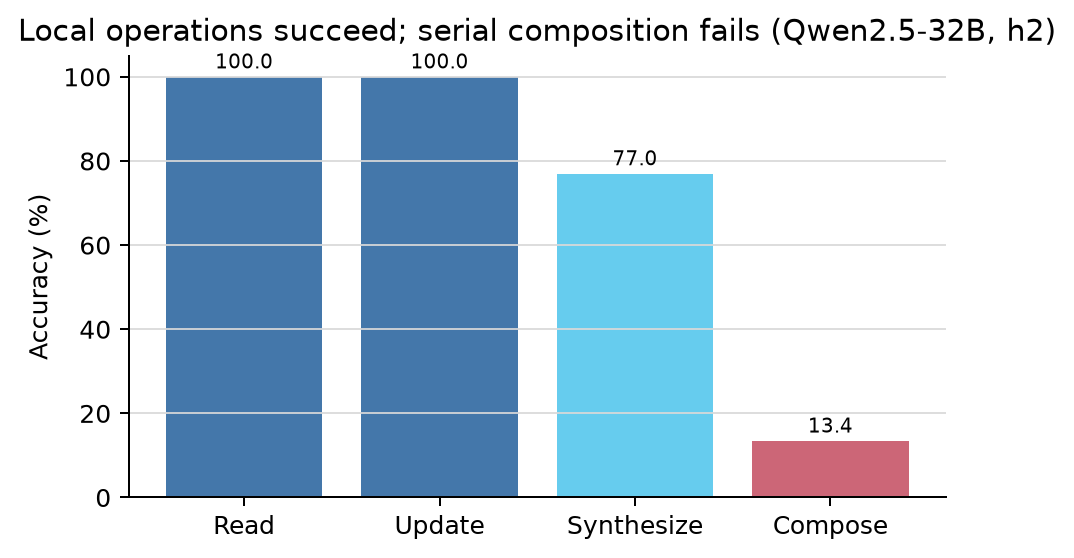
\includegraphics[width=.72\linewidth]{01_native_factorization.png}
\caption{Frozen Qwen2.5-32B at horizon two. All 1,920 cases pass the local
competence controls, yet Compose remains near eight-state chance.}
\label{fig:diagnosis}
\end{figure}

Figure~\ref{fig:diagnosis} shows the main diagnosis. At h2, Synthesize reaches
76.98\% while Compose reaches 13.44\%. Among cases where Read, Update, and
Synthesize all succeed, Compose remains 13.59\%. This is a routing failure, not
an absence of the local operation.

\subsection{Explicit state handoff repairs the immediate failure}

\begin{figure}[t]
\centering
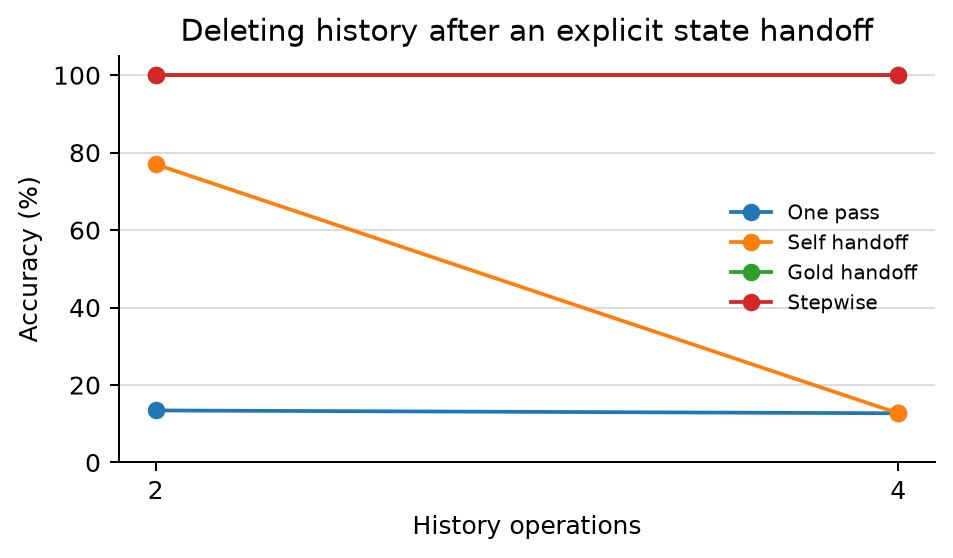
\includegraphics[width=.72\linewidth]{02_explicit_handoff.png}
\caption{A second call receives only the state and final rule. Gold and
stepwise conditions show that state use and local updates are available.}
\label{fig:handoff}
\end{figure}

At h2, model self-handoff matches state synthesis at 76.98\%, a +63.54 point
gain over one-pass Compose. Gold handoff and stepwise decimal execution are
perfect. At h4, state synthesis itself falls to chance, so self-handoff cannot
repair the upstream error.

\subsection{Rate limits recovery and redundant rate improves reliability}

\begin{figure}[t]
\centering
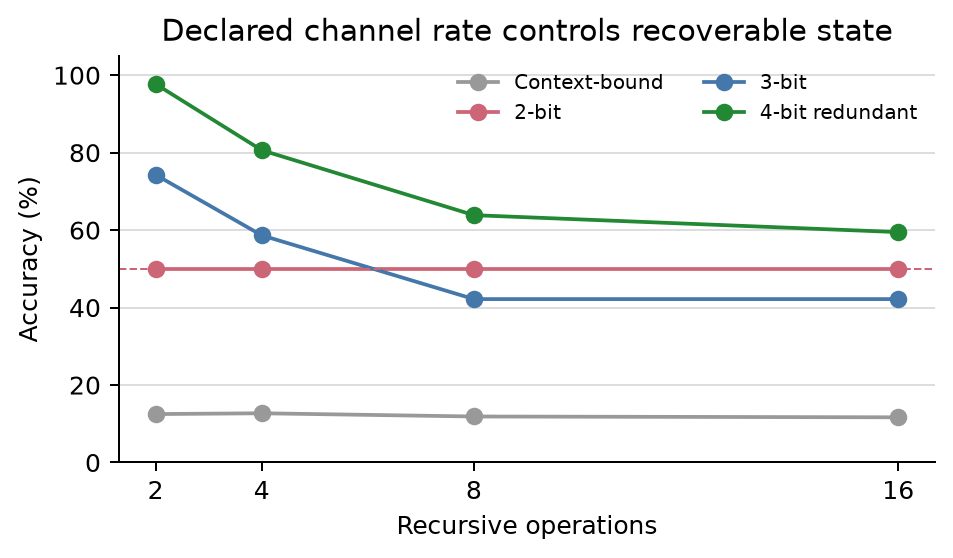
\includegraphics[width=.72\linewidth]{03_rate_capacity.png}
\caption{One-token channels with declared rates of two, three, and four bits
for an eight-state task. The two-bit channel reaches its exact 50\% ceiling.}
\label{fig:rate}
\end{figure}

The two-bit channel maps pairs of states to the same code and reaches exactly
50\% answer accuracy at every horizon. The context-bound control remains near
12.5\%, despite having enough surface symbols, showing that a shared dictionary
matters. Gold-code swaps preserve same-state behavior and transfer
different-state behavior for the canonical and redundant codes.

\subsection{Closure, not endpoint fit, drives long-horizon reuse}

\begin{figure}[t]
\centering
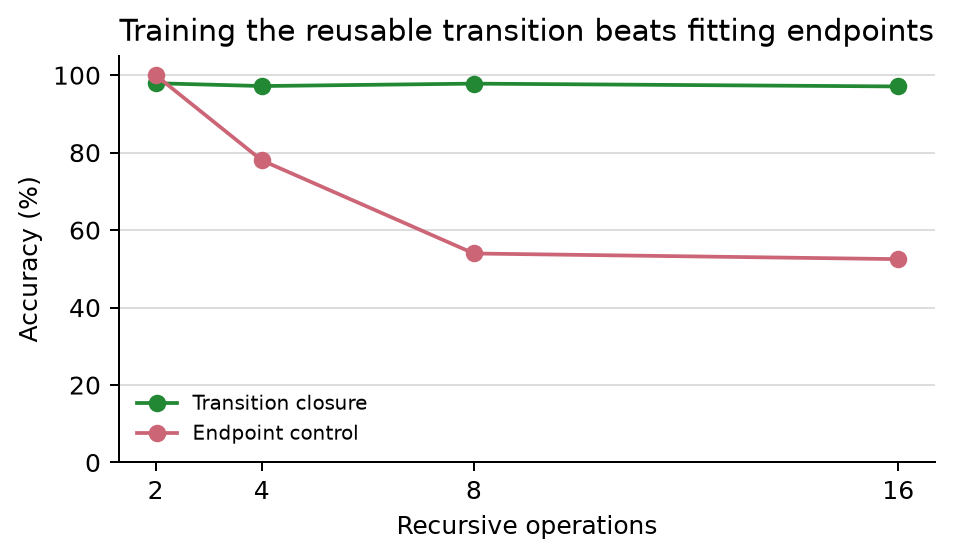
\includegraphics[width=.72\linewidth]{04_closure_training.png}
\caption{Matched training compute; only the producer target differs.}
\label{fig:closure}
\end{figure}

At h8 and h16, redundant closure beats endpoint training by 43.85 and 44.58
points, with program-context bootstrap intervals excluding zero. Under five
history shifts, closure retains 93.25\% mean h16 accuracy versus 48.50\% for
the endpoint control. This rules out a single positional history template, but
not overfitting to the finite addition transition family.

\begin{figure}[t]
\centering
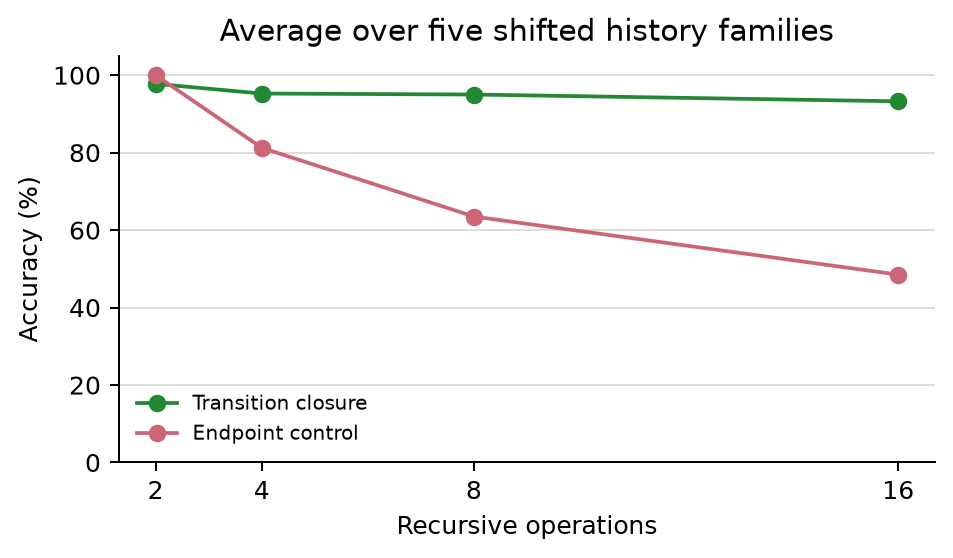
\includegraphics[width=.72\linewidth]{05_distribution_shift.png}
\caption{Mean accuracy across structured, IID, shuffled, cancellation, and
repeated-operation histories. Each cell has five program contexts.}
\label{fig:stress}
\end{figure}

\subsection{Local reliability is not global reliability}

\begin{figure}[t]
\centering
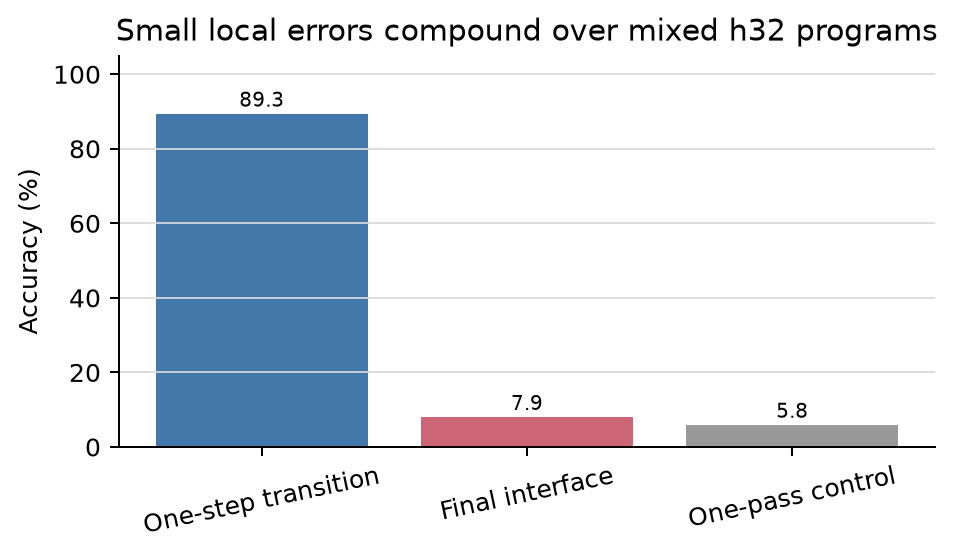
\includegraphics[width=.72\linewidth]{06_local_global_reliability.png}
\caption{Three Qwen seeds on held-out mixed register programs at h32. The
one-step score conditions on the state code the model actually received.}
\label{fig:register}
\end{figure}

The register confirmation fails its preset gate. Conditional transition
accuracy is 89.31\%, but complete interface accuracy is 7.92\%, against 5.83\%
one-pass and 6.25\% chance. The programs contain about 24 real state changes.
An extra channel bit raises two completed seeds to only 12.81\% and 12.19\%.
Redundancy cannot compensate for a transition kernel that is not reliable
enough under mixed recursive use.

\begin{figure}[t]
\centering
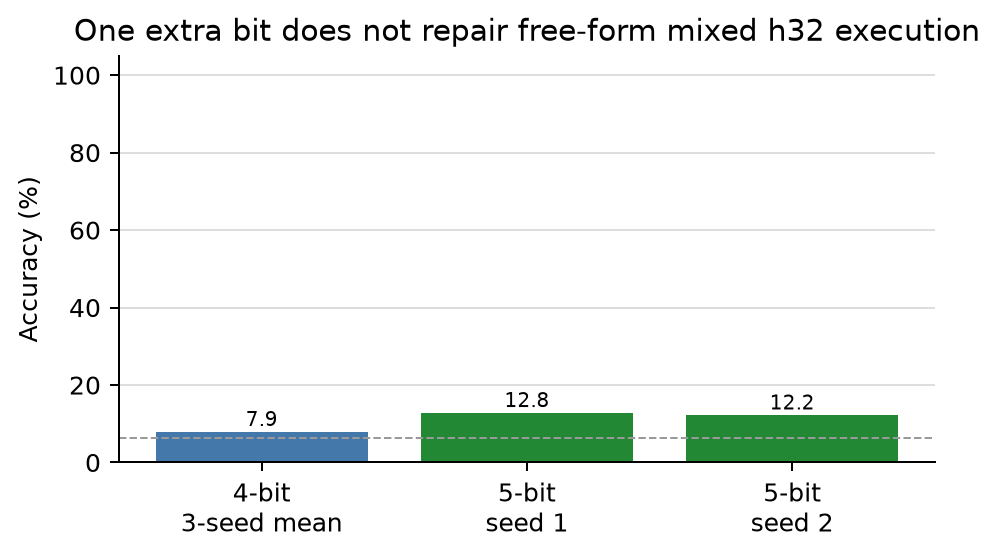
\includegraphics[width=.72\linewidth]{08_register_redundancy_negative.png}
\caption{Held-out mixed h32 register accuracy. The third five-bit seed has no
complete summary and is excluded. The dashed line is 16-state chance.}
\label{fig:register-rate}
\end{figure}

\subsection{Proof-state pilot}

\begin{figure}[t]
\centering
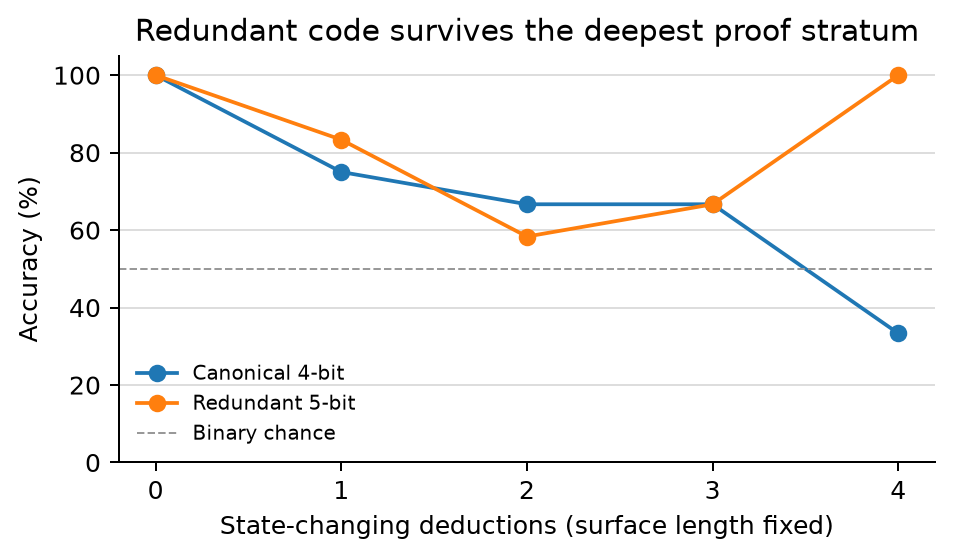
\includegraphics[width=.72\linewidth]{07_proof_active_depth.png}
\caption{Fixed 64-rule surface length; each point has 12 cases.}
\label{fig:proof}
\end{figure}

The redundant five-bit proof interface is 81.67\% overall and reaches 100\% at
four active deductions, versus 75\% one-pass. Canonical four-bit accuracy falls
to 33.33\% in the same stratum. This is consistent with redundancy improving
recursive reliability, but the small, non-monotone strata do not yet establish
a rate--reliability law for proof.

\section{Relation to latent state and long-horizon reasoning}

\citet{chen2024states} show that models can form implicit discrete state
representations and use them in arithmetic. We test a different boundary:
whether state information is organized as a reusable interface. Our frozen
model result shows that local decoding and local manipulation do not imply
serial routing. Our trained result shows that an explicit channel can acquire
sufficiency and closure. The register failure shows why long-horizon reasoning
needs more than state identification: if each self-conditioned update succeeds
with probability below one, error compounds with effective transition depth.

This suggests that reasoning trajectories should be studied at three levels:
representation geometry, semantic state, and interface dynamics. Geometry asks
where information appears. State asks which histories are equivalent for the
future. Interface dynamics asks whether the model can repeatedly move between
those equivalence classes without leaving them.

\section{Limitations and falsifiers}

The strongest result uses finite synthetic addition. The proof result has 12
cases per depth and one model checkpoint. The register result is a negative
confirmation, not a repair. We do not claim that ordinary language models
naturally expose discrete state tokens, that extra capacity always helps, or
that the method yet improves open-domain reasoning.

The main claim would weaken if matched closure controls reproduced the gain,
if independently trained consumers could not use the codes, if code swaps did
not transfer state-dependent behavior, or if the rate ceiling failed under
balanced states. Broad reasoning claims require tasks where the sufficient
state is not supplied by the benchmark designer.

\section{Next experiments}

\begin{enumerate}
  \item Confirm the proof-depth comparison over at least 30 contexts and three
  seeds, balancing target states within each active-depth stratum.
  \item Train mixed-operation register transitions to a preset local reliability
  target before evaluating horizon, then compare observed end accuracy with a
  measured error-propagation model.
  \item Test proof search, program execution, and planning tasks with explicit
  sufficient-state definitions and held-out transition compositions.
  \item Connect token interfaces to latent trajectories by measuring when a
  hidden trajectory becomes predictive of the emitted quotient state and
  whether interventions at that point change the code.
\end{enumerate}

\section{Reproducibility}

The paper workspace's \texttt{evidence.json} maps every plotted number to its
saved JSON source. Complete and partial runs remain separate. Data generation
uses fixed seeds, hashed program files, group-disjoint contexts, exact symbolic
verification, and program-context bootstrap intervals. No LLM judge scores
these tasks.

\bibliographystyle{plainnat}
\bibliography{references}
\end{document}
